\section{CPN Analysis Model}
\label{sec:CPN}

%\begin{figure}[h]
%	\centering
%	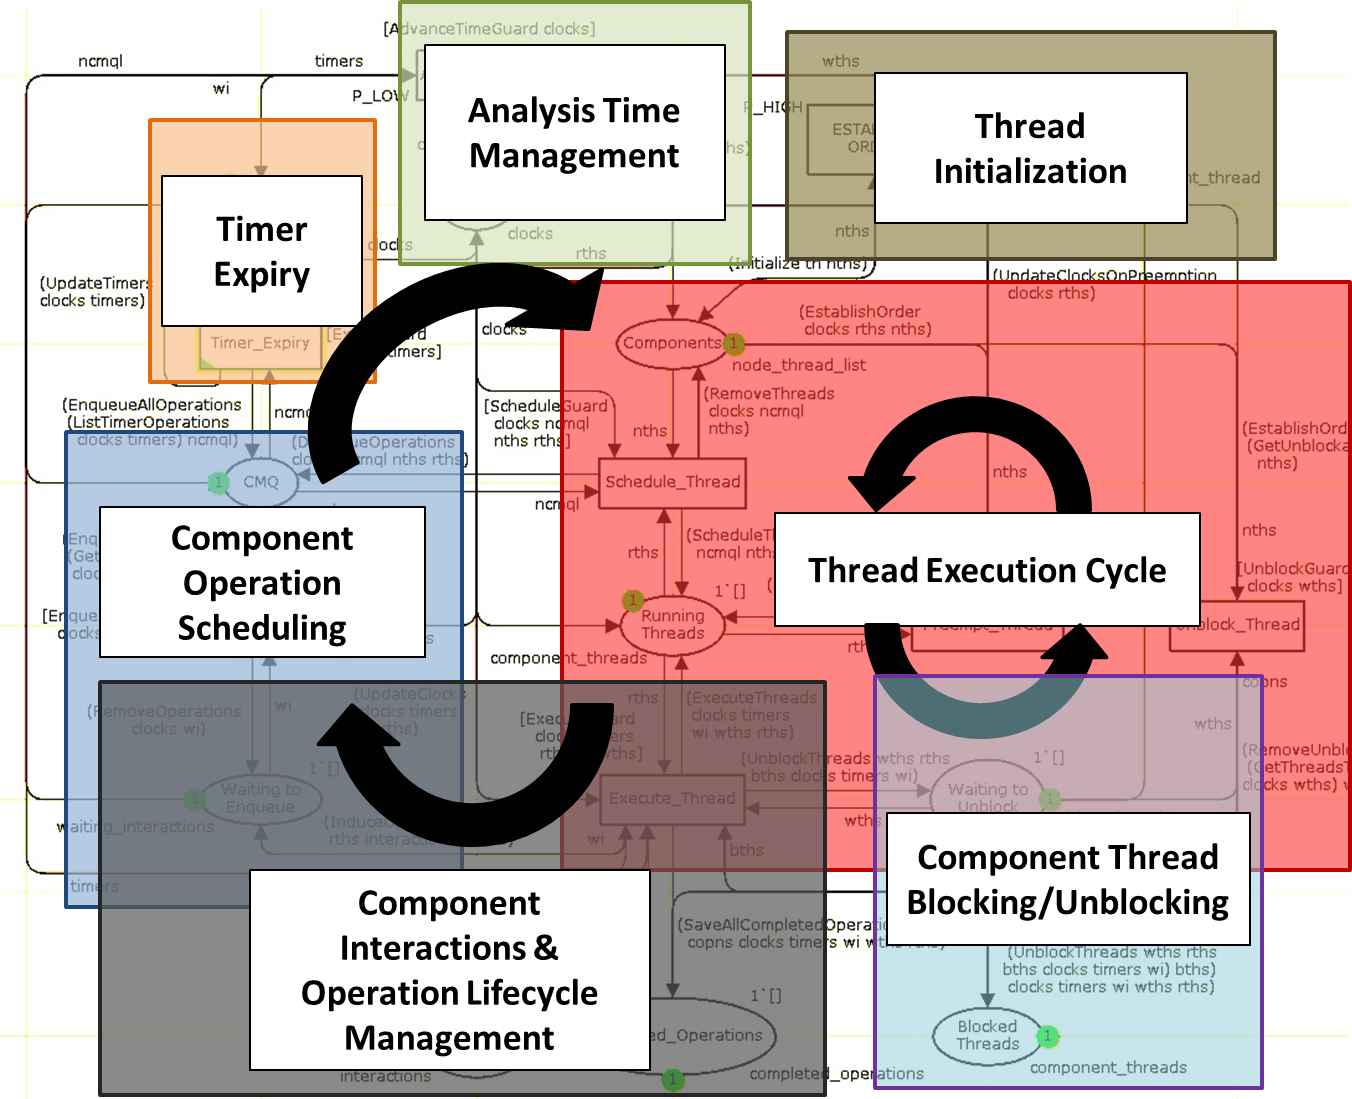
\includegraphics[width=0.4\textwidth]{hlcpn_structure}
%	\caption{Structural Aspects}
%	\label{fig:hlcpn_structure}
%\end{figure}

For the sake of brevity, a detailed description of both Colored Petri nets and our timing analysis model are not within the scope of this paper. The CPN analysis model consists of a collection of interacting sub-models, each responsible for modeling and simulating specific sub-systems in an application lifecycle e.g. thread scheduling, operation scheduling, thread execution, blocking and waiting times, timer expiries, and time progression. From the design model of the system, we generate the initial CPN tokens that are injected into places in this analysis model. Using the in-built state space analysis engine, we analyze the state space of the parameterized model to compute useful system properties \cite{kumar2014colored} \cite{SEUS} e.g. processor utilization, execution time plots, deadline violations etc.   




